\documentclass[pdftex,12pt,a4paper]{article}

\usepackage{graphicx}  
\usepackage[margin=2.5cm]{geometry}
\usepackage{breakcites}
\usepackage{indentfirst}
\usepackage{pgfgantt}
\usepackage{pdflscape}
\usepackage{float}
\usepackage{epsfig}
\usepackage{epstopdf}
\usepackage[cmex10]{amsmath}
\usepackage{stfloats}
\usepackage{multirow}

\renewcommand{\refname}{REFERENCES}
\linespread{1.3}

\usepackage{mathtools}
%\newcommand{\HRule}{\rule{\linewidth}{0.5mm}}
\thispagestyle{empty}
\begin{document}
\begin{titlepage}
\begin{center}
\textbf{}\\
\textbf{\Large{ISTANBUL TECHNICAL UNIVERSITY}}\\
\vspace{0.5cm}
\textbf{\Large{COMPUTER ENGINEERING DEPARTMENT}}\\
\vspace{4cm}
\textbf{\Large{BLG 222E\\ COMPUTER ORGANIZATION\\ PROJECT 2 REPORT}}\\
\vspace{4cm}
\begin{table}[ht]
\centering
\Large{
\begin{tabular}{lcl}
\textbf{CRN}  & : & 21335 \\
\textbf{LECTURER}  & : & Prof. Dr. Deniz Turgay Altılar \\
\end{tabular}}
\end{table}
\vspace{1cm}
\textbf{\Large{GROUP MEMBERS:}}\\
\begin{table}[ht]
\centering
\Large{
\begin{tabular}{rcl}
150210077  & : & Emre Yamaç \\
150210088  & : & Alper Tutum \\
\end{tabular}}
\end{table}
\vspace{2.8cm}
\textbf{\Large{SPRING 2024}}

\end{center}

\end{titlepage}

\thispagestyle{empty}
\addtocontents{toc}{\contentsline {section}{\numberline {}FRONT COVER}{}}
\addtocontents{toc}{\contentsline {section}{\numberline {}CONTENTS}{}}
\setcounter{tocdepth}{4}
\tableofcontents
\clearpage

\setcounter{page}{1}

\section{INTRODUCTION}
In the second project of the computer organization course, we took on the task of designing a basic Central Processing Unit (CPU). The main purpose requested from us in this project was to carry out the instructions given to us by applying the necessary operations at the appropriate time, by using the Address Register File, Register File, Instruction Register, ALU, Memory and necessary Registers that we created in the previous project. After following the instructions, we simulated our instructions and compared the situations as a result of the appropriate operations in the RAM.mem file.

\section{MATERIALS AND METHODS}
In this section, the implementation details of the CPU System are
explained.

\subsection{Sequence Counter}
A sequence counter for the CPU is implemented by creating a 3-bit
register 'SC' and by initializing its value to 0. SC is incremented
with each negative edge of the clock and the next time signal is
obtained by decoding SC to an 8 bit 'T' register.

\begin{table}[H]
\centering
\begin{tabular}{|c|c|}
  \hline
  SC & T\\
  \hline
  000 & 00000001\\
  \hline
  001 & 00000010\\
  \hline
  010 & 00000100\\
  \hline
  011 & 00001000\\
  \hline
  100 & 00010000\\
  \hline
  101 & 00100000\\
  \hline
  110 & 01000000\\
  \hline
  111 & 10000000\\
  \hline
\end{tabular}
\caption{Decoding of Sequence Counter\cite{ref1}}
\end{table}

The sequence counter counts from 0 to 7 as long as it is not cleared
by two particular signals. One of the signals is 'Reset'. It is an
external signal which stops the sequence counter when its value is
0. The other signal comes from the 'CLR' flip-flop which is set when
an instruction reaches its end.

\subsection{Arithmetic Logic Unit System}
The Arithmetic Logic Unit System implemented in the previous project is
used without making any changes to the module definition. To summarize
the ALU System consists of an ALU, Register File, Address Register
File, Instruction Register, Memory Unit, and three multiplexers.

\begin{figure}[H]
	\centering
	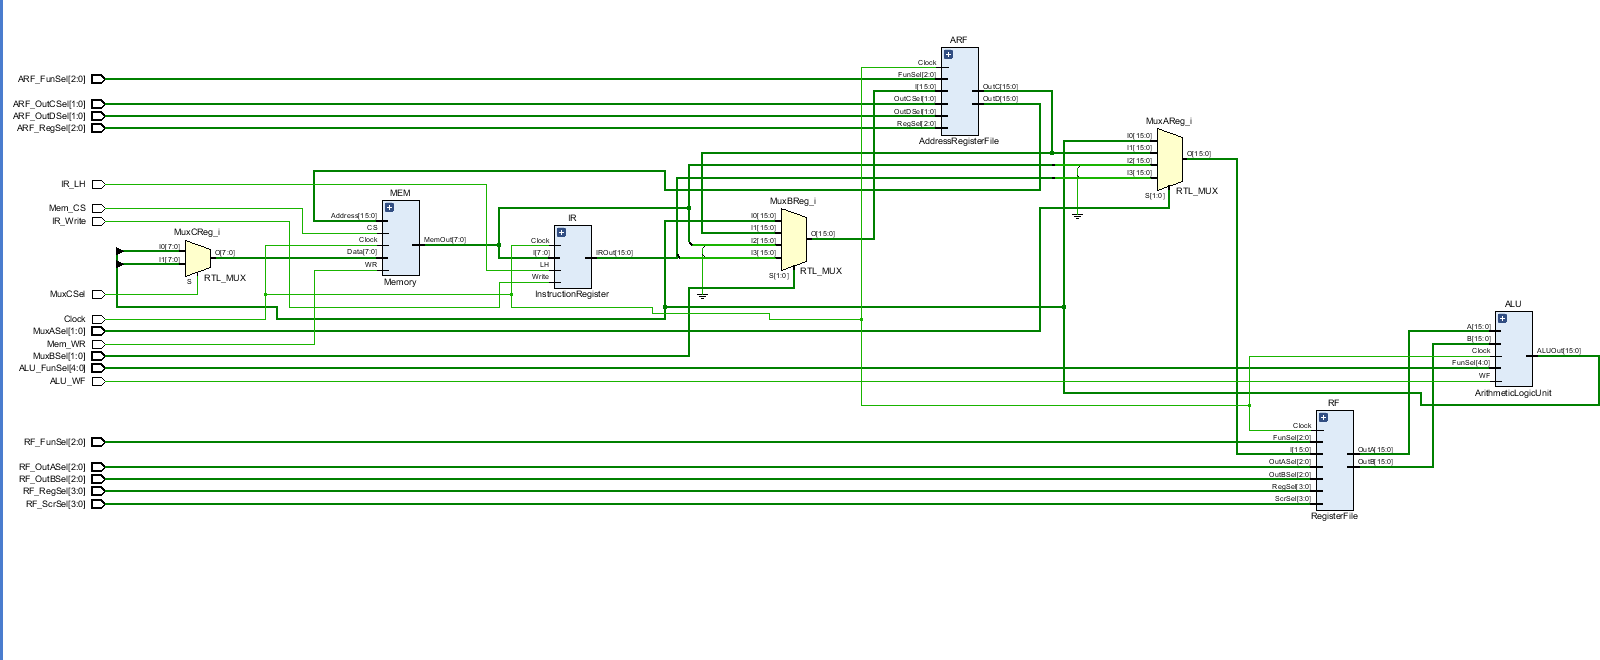
\includegraphics[width=0.5\textwidth]{1.png}	
	\caption{Schematic of ALU System\cite{ref1}}
	\label{fig1}
\end{figure}

Every select input of the module is connected to reg variables in the
CPU for controlling the flow of data in the system. The data output
of the Instruction Register inside the ALU System is assigned to a
variable 'IR' since it will later be used for the fetch & decode phase.
Every register in the Register File and Address Register File is
initialized to 16-bit 0 except for SP in ARF. The Stack Pointer starts
from 255 which is the bottom address of the given RAM.

\subsection{Fetch and Decode}
The fetch and decode procedure is designed to happen in two clock
cycles. This is because the memory unit holds 8 bit data. In the first
clock cycle, the ram data that the Program Counter (PC) is pointing to
is written on the LSB 8 bits of the Instruction Register and PC is
incremented by one. In the second clock cycle the memory data is
written to MSB 8 bits of IR and PC is incremented again so that it
points to the next instruction.

The instruction format of the given design is explained below:

\begin{table}[H]
\centering
\begin{tabular}{|c|c|c|}
  \hline
  OPCODE (6-bit) & Rsel (2-bit) & Address (8-bit)\\
  \hline
\end{tabular}
\caption{Memory Reference Instruction Format\cite{ref1}}
\end{table}

Memory reference instructions select a general purpose register from
RF and use it for reading or writing. Some instructions don't use the
selected register at all.

\begin{table}[H]
\centering
\begin{tabular}{|c|c|}
  \hline
  Rsel & Selected Register\\
  \hline
  00 & R1\\
  \hline
  01 & R2\\
  \hline
  10 & R3\\
  \hline
  11 & R4\\
  \hline
\end{tabular}
\caption{Register select of memory reference instructions\cite{ref1}}
\end{table}

\begin{table}[H]
\centering
\begin{tabular}{|c|c|c|c|c|}
  \hline
  OPCODE (6-bit) & S & DSTREG & SREG1 & SREG2\\
  \hline
\end{tabular}
\caption{Register Reference Instruction Format\cite{ref1}}
\end{table}

\begin{table}[H]
\centering
\begin{tabular}{|c|c|}
  \hline
  DSTREG/SREG1/2 & Selected Register\\
  \hline
  000 & PC\\
  \hline
  001 & PC\\
  \hline
  010 & SP\\
  \hline
  011 & AR\\
  \hline
  100 & R1\\
  \hline
  101 & R2\\
  \hline
  110 & R3\\
  \hline
  111 & R4\\
  \hline
\end{tabular}
\caption{Register select of register reference instructions\cite{ref1}}
\end{table}

In this project's design, a flip-flop 'M' is defined for distinguishing
between memory reference instructions and non-memory reference
instructions in the decoding phase. The decoding of IR happens during
every cycle after the first two.

\underline{If memory reference:}
Either OutASel or RegSel of RF should be set depending on the
instruction. In the proposed design, Mem WR is checked in the decode
block in order to decide if a memory read or write operation is
taking place. If the operation is a memory write, OutASel is set to
give the selected register into the ALU and ALU FunSel is set to
directly feed the contents of the selected register to its output
which is connected to Memory via a MUX. If the operation is a memory
read, the contents of the register is likely to change so RegSel of RF
is set depending on the Rsel bits of IR before going to the execution
phase. If the operation is a memory read operation but the Rsel bits
are unnecessary, the RegSel is blocked exclusively inside the
definition of the instruction.

\underline{If register reference:}
DSTREG bits of IR are decoded and RegSel of RF and ARF are set
accordingly. SREG1 and SREG2 bits are decoded to select what is fed 
into OutA and OutB of RF respectively. Additionally, an S bit exists
in this type of instruction. It is directly connected to the WF input
of ALU. If 1, it means the flags of ALU can change.

\subsection{Execution of Instructions}
The OPCODE part from IR was read and a case was written for every
defined instruction. Each case was then divided into its clock signals.
Inside the cases, every control signal that allows the required
register transfer is set. Since the decoding part deals with choosing
which registers to write or read, there is no need for extra cases
inside of the OPCODE cases.

\section{RESULTS}
The results for some instructions are given below. The instructions
are chosen from the example outputs given to us. As shown below, the
outputs we received match the example outputs.

\subsection{Fetch & Decode}
\begin{figure}[H]
	\centering
	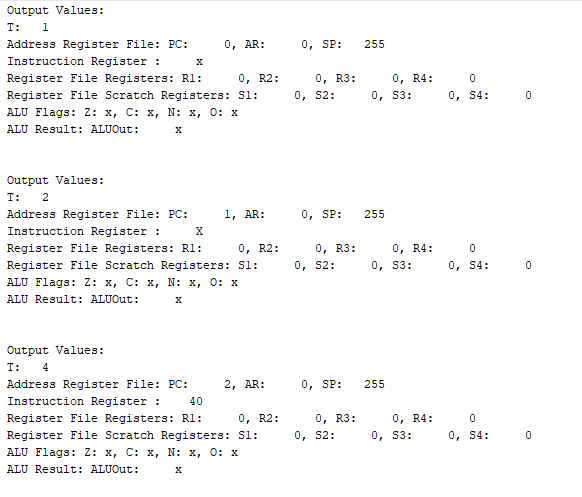
\includegraphics[width=0.5\textwidth]{bra1.png}	
	\label{fig2}
\end{figure}

\subsection{BRA}
\begin{figure}[H]
	\centering
	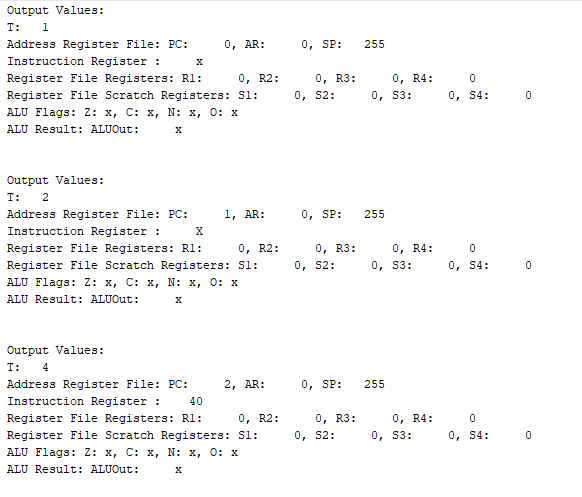
\includegraphics[width=0.5\textwidth]{bra1.png}	
	\label{fig3}
\end{figure}
\begin{figure}[H]
	\centering
	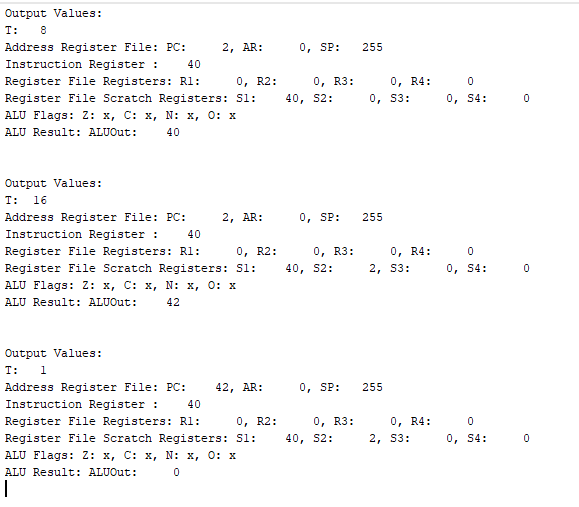
\includegraphics[width=0.5\textwidth]{bra2.png}	
	\label{fig4}
\end{figure}

\subsection{DEC}
\begin{figure}[H]
	\centering
	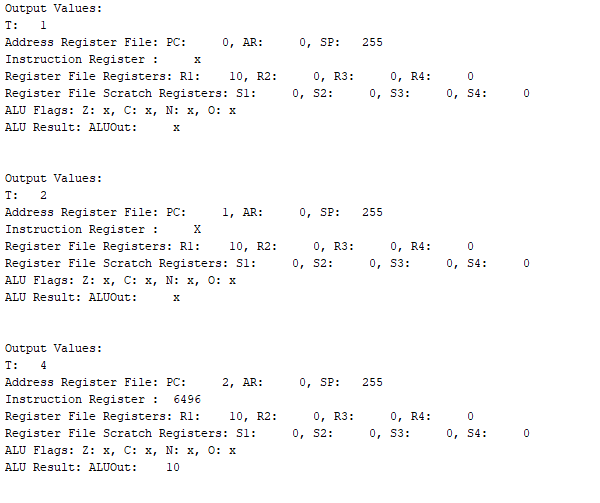
\includegraphics[width=0.5\textwidth]{dec1.png}	
	\label{fig5}
\end{figure}
\begin{figure}[H]
	\centering
	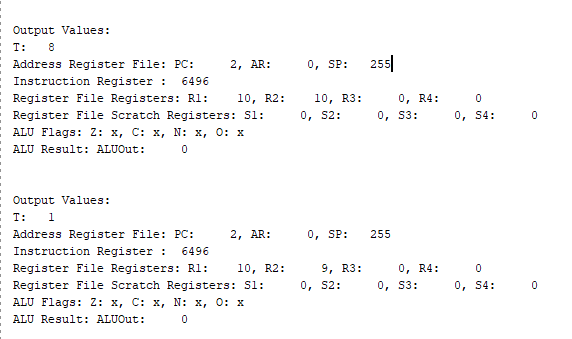
\includegraphics[width=0.5\textwidth]{dec2.png}	
	\label{fig6}
\end{figure}

\subsection{INC}
\begin{figure}[H]
	\centering
	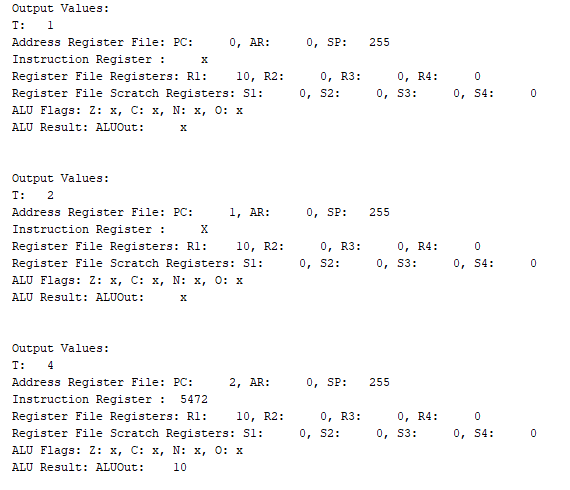
\includegraphics[width=0.5\textwidth]{inc1.png}	
	\label{fig7}
\end{figure}
\begin{figure}[H]
	\centering
	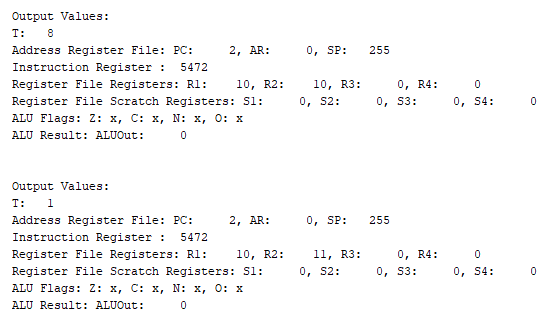
\includegraphics[width=0.5\textwidth]{inc2.png}	
	\label{fig8}
\end{figure}

\subsection{MOVH}
\begin{figure}[H]
	\centering
	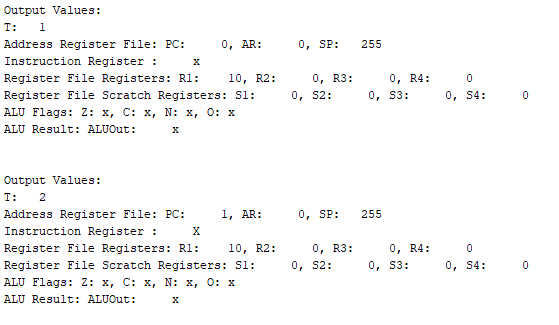
\includegraphics[width=0.5\textwidth]{movh1.png}	
	\label{fig9}
\end{figure}
\begin{figure}[H]
	\centering
	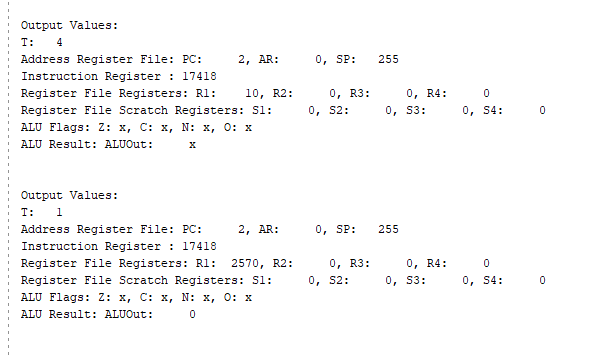
\includegraphics[width=0.5\textwidth]{movh2.png}	
	\label{fig10}
\end{figure}

\subsection{MOVL}
\begin{figure}[H]
	\centering
	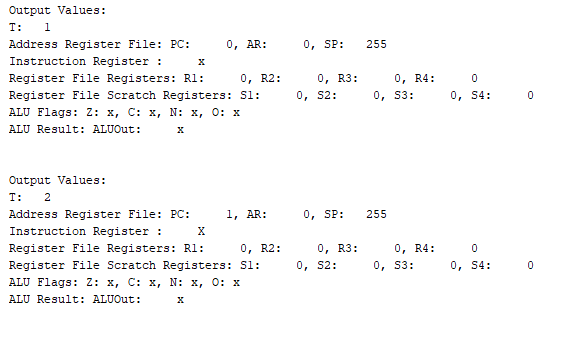
\includegraphics[width=0.5\textwidth]{movl1.png}	
	\label{fig11}
\end{figure}
\begin{figure}[H]
	\centering
	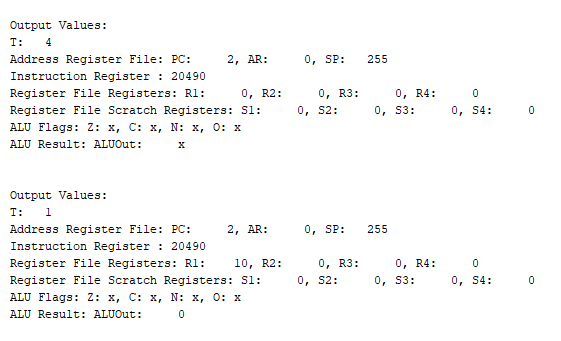
\includegraphics[width=0.5\textwidth]{movl2.png}	
	\label{fig12}
\end{figure}

\subsection{XOR}
\begin{figure}[H]
	\centering
	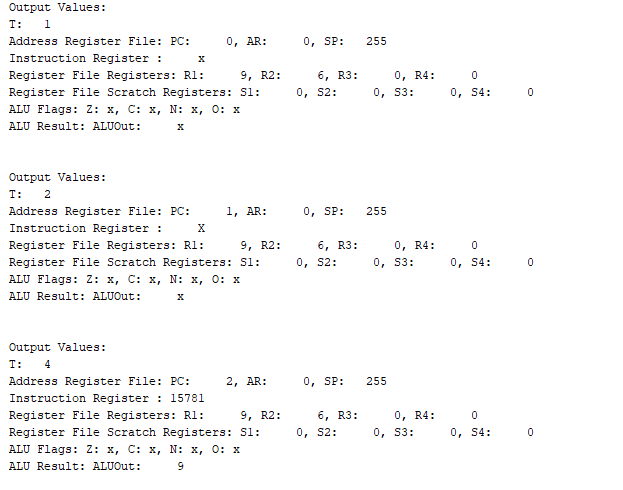
\includegraphics[width=0.5\textwidth]{xor1.png}	
	\label{fig13}
\end{figure}
\begin{figure}[H]
	\centering
	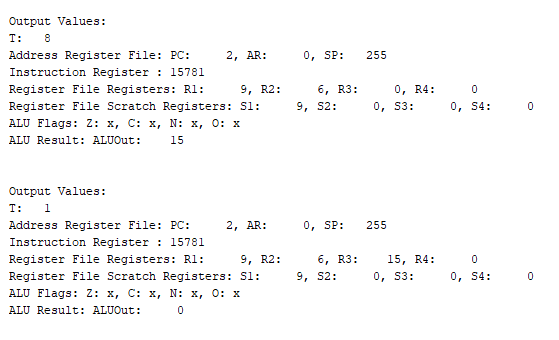
\includegraphics[width=0.5\textwidth]{xor2.png}	
	\label{fig14}
\end{figure}

\section{DISCUSSION}
In this project, we successfully managed to implement our own CPU
design using the ALU System we created before. Our first step was to
solve the remaining issues in the previous project so that the errors
aren't carried into this project. Then we designed the CPU on paper and
noted every single register transfer in each time cycle of every single
instruction. This made things a lot easier for us. By looking at the
paper we wrote our verilog code for each instruction. We specified
every control for every operation and it took great time. Since
there was a big chunk of code we faced lots of problems with our
coding and debugged to solve the errors that didn't let us compile.
Then we tested fetch & decode and every instruction given in the pdf
one by one. As a result we had all of the instructions working as
expected, at least on their own. However we faced some issues when
using the instructions in sequence. The example program worked only
partially, the first iteration of the program loop went smoothly but
after that it was broken. The problem is most likely with the ram.mem
file since we didn't have much time for testing the example program.
At least that's what we assume since the first iteration of the loop
goes perfectly and then different operations take place in the second
iteration. As a conclusion, the biggest difficulty in this project for
us was not allocating enough time for testing.

\section{CONCLUSION}
To summarize, in our project, we first wrote on a piece of paper which actions the instructions would perform according to time, and drafted the necessary control signals by drawing it to the template of Part 4 we made in the last project. Afterwards, we defined the necessary cables and registers in Verilog and wrote the process of uploading to IR. We defined the opcodes according to the time cycle sketch we created, and after controlling the necessary signals, we finally simulated and compared our answers with the example outputs.

\newpage
\addcontentsline{toc}{section}{\numberline {}REFERENCES}

\bibliographystyle{unsrt}
\bibliography{reference}

\end{document}

